\chapter{Desktop-Anwendung}
\label{chap:DesktopAnwendung}

\section{Notification Area}
Als Notification Area werden alle rechtsbündigen Symbole bis zu dem Pfeil, der nach oben zeigt bezeichnet, wenn man auf den Pfeil klickt wird die Overflow Area geöffnet. In diesen Bereich werden standardmäßig einige Symbole verschoben. Jedes Symbol kann von der Notification Area in die Overflow Area verschoben werden dasselbe gilt auch für die andere Richtung
\begin{figure}[H]
    \centering
    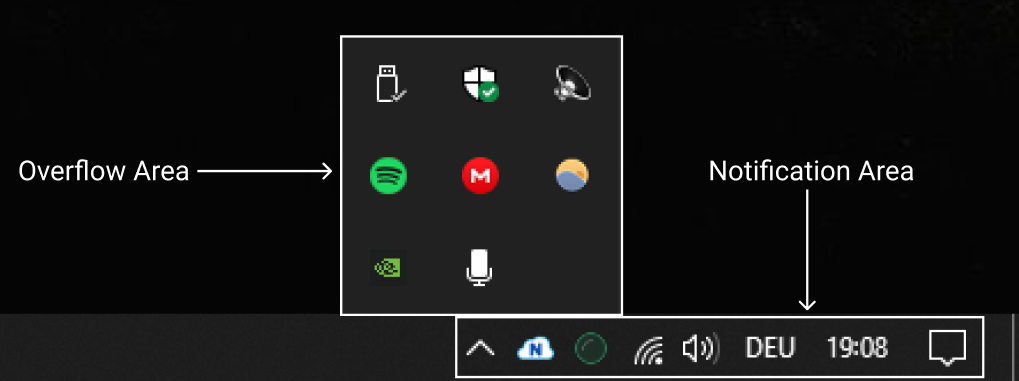
\includegraphics[width=0.8\textwidth]{NotificationArea.png}
    \caption[NotificationArea]{Notification Area} 
\end{figure}
\  \\
Die Notification Area ist besser bekannt unter dem Namen Systemtray, wird aber offiziell von Windows als Notification Area bezeichnet. Der Begriff Systemtray kommt von Windows 95, weil es da eine Anwendung gibt die systray.exe heißt, nachdem dieses Programm geschlossen wurde sind die Symbole die in der Notification Area angezeit wurden verschwunden. Deshalb hat man angenommen, da die Anwendung die dafür zuständig ist systray.exe heißt, dann ist der Name des Bereichs wo die Symbole angezeigt werden sicher Systemtray. Das ist aber nicht der einzige Grund der Verwirrung gewesen Microsoft Mitarbeiter haben den Bereich als Systemtray bezeichnet und bis 2003 war auch in der Windows Dokumentation der Begriff Systemtray enthalten. Unter WIndows 10 noch zu finden

\subsection{Windows Guidelines}
Dieser Bereich wurde Notification Area genannt, da der Plan war das nur Symbole gezeigt werden, die dem Benutzer hilfreiche Informationen geben entweder anhand von Benachrichtigungen oder das sich das Symbol ändert wie zum Beispiel bei der Akkustandanzeige. Ein anderer wichtiger Aspekt eines Symbols in der Notification Area ist, das die Information wichtig genug ist den Benutzer zu stören, trotzdem aber keine sofortige  Benutzeraktion erfordert. Die Benachrichtigungen sollen ohne weiteres einfach ignoriert werden können, falls es doch eine Wichtige 

\subsection{Position}

\subsection{Anwendung}

\section{Kommunikation zwischen Treiber und Anwendung}
\subsection{Starten}